%%% LaTeX Template: Article/Thesis/etc. with colored headings and special fonts
%%%
%%% Source: http://www.howtotex.com/
%%% Feel free to distribute this template, but please keep to referal to http://www.howtotex.com/ here.
%%% February 2011
%%%
%%% Modified May 2018 by CDM

%%%  Preamble
\documentclass[11pt,letterpaper]{article}
\usepackage[margin=1.0in]{geometry}
\usepackage[T1]{fontenc}
\usepackage[bitstream-charter]{mathdesign}
\usepackage[latin1]{inputenc}					
\usepackage{amsmath}						
\usepackage{xcolor}
\usepackage{cite}
\usepackage{hyphenat}
\usepackage{graphicx}
\usepackage{float}
\usepackage{subfigure}
\usepackage{sectsty}
\usepackage[compact]{titlesec} 
\usepackage[tablegrid]{vhistory}
\allsectionsfont{\color{accentcolor}\scshape\selectfont}

%%% Definitions
\definecolor{accentcolor}{rgb}{0.0,0.0,0.5} 
\newcommand{\teamname}{Team Name}
\newcommand{\productname}{Product Name}
\newcommand{\coursename}{CSE 4316: Senior Design I}
\newcommand{\semester}{Spring 2018}
\newcommand{\docname}{System Requirements Specification}
\newcommand{\department}{Department of Computer Science \& Engineering}
\newcommand{\university}{The University of Texas at Arlington}
\newcommand{\authors}{Alan Turing \\ Grace Hopper \\ John Von Neumann \\ Ada Lovelace \\ Charles Babbage}

%%% Headers and footers
\usepackage{fancyhdr}
	\pagestyle{fancy}						% Enabling the custom headers/footers
\usepackage{lastpage}	
	% Header (empty)
	\lhead{}
	\chead{}
	\rhead{}
	% Footer
	\lfoot{\footnotesize \teamname \ - \semester}
	\cfoot{}
	\rfoot{\footnotesize page \thepage\ of \pageref{LastPage}}	% "Page 1 of 2"
	\renewcommand{\headrulewidth}{0.0pt}
	\renewcommand{\footrulewidth}{0.4pt}

%%% Change the abstract environment
\usepackage[runin]{abstract}			% runin option for a run-in title
%\setlength\absleftindent{30pt}			% left margin
%\setlength\absrightindent{30pt}		% right margin
\abslabeldelim{\quad}	
\setlength{\abstitleskip}{-10pt}
\renewcommand{\abstractname}{}
\renewcommand{\abstracttextfont}{\color{accentcolor} \small \slshape}	% slanted text

%%% Start of the document
\begin{document}

%%% Cover sheet
{\centering \huge \color{accentcolor} \sc \textbf{\department \\ \university} \par}
\vspace{1 in}
{\centering \huge \color{accentcolor} \sc \textbf{\docname \\ \coursename \\ \semester} \par}
\vspace{0.5 in}
\begin{figure}[h!]
	\centering
   	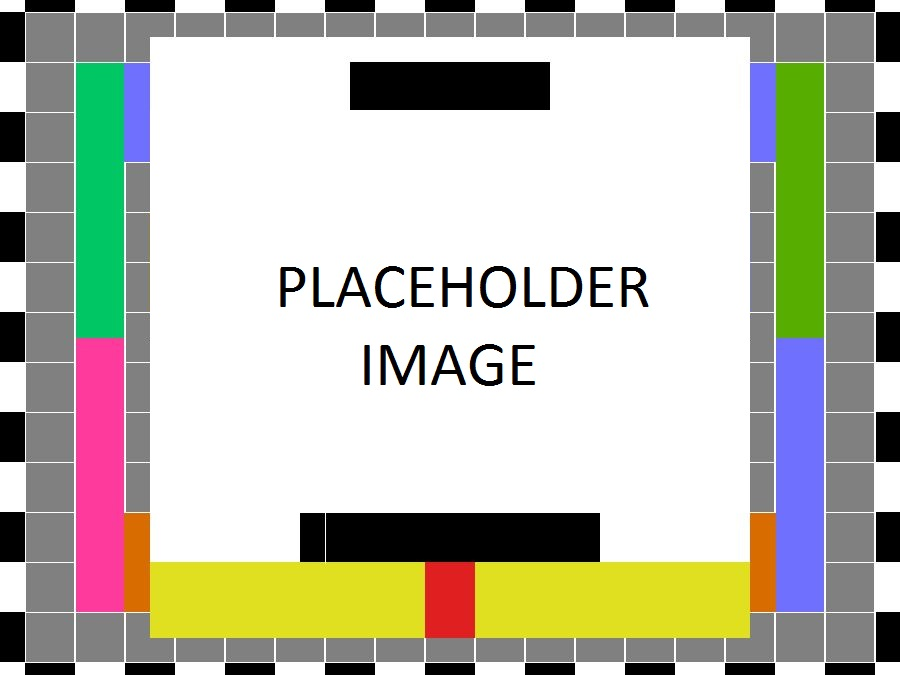
\includegraphics[width=0.60\textwidth]{images/test_image}
\end{figure}
\vspace{0.5 in}
{\centering \huge \color{accentcolor} \sc \textbf{\teamname \\ \productname} \par}
\vspace{0.5 in}
{\centering \large \sc \textbf{\authors} \par}
\newpage


%\vspace{1 in}
%\centerline{January 13th, 2012}
%\newpage

%%% Revision History
\begin{versionhistory}
  	\vhEntry{0.1}{10.01.2015}{GH}{document creation}
  	\vhEntry{0.2}{10.05.2015}{AT|GH}{complete draft}
  	\vhEntry{0.3}{10.12.2015}{AT|GH}{release candidate 1}
  	\vhEntry{1.0}{10.20.2015}{AT|GH|CB}{official release}
  	\vhEntry{1.1}{10.31.2015}{AL}{added customer change requests}
\end{versionhistory}
\newpage

%%% Table of contents
\setcounter{tocdepth}{3}
\tableofcontents
\newpage

%%% List of figures and tables (optional)
\listoffigures
%\listoftables
\newpage

\section{Product Concept}
This section describes the purpose, use and intended user audience for the sound backpack product. The sound backpack is a system that takes in musical sound waves and outputs them as vibrations. The sound backpack will allow users with hearing disabilities to enjoy music by allowing them to fill the sound waves of songs.

\subsection{Purpose and Use}
The sound backpack will take in a song, filter the low, mid, and high frequencies, then pass those frequencies to different shakers inside the backpack. The shakers will emit a vibration in time with the music so users can feel the beat.

\subsection{Intended Audience}
The sound backpack will be available for purchase by the general public, but it will be designed and targeted for customers with hearing disabilities. Age restrictions may apply after evaluating the complexity of the final product.

\begin{figure}[h!]
	\centering
   	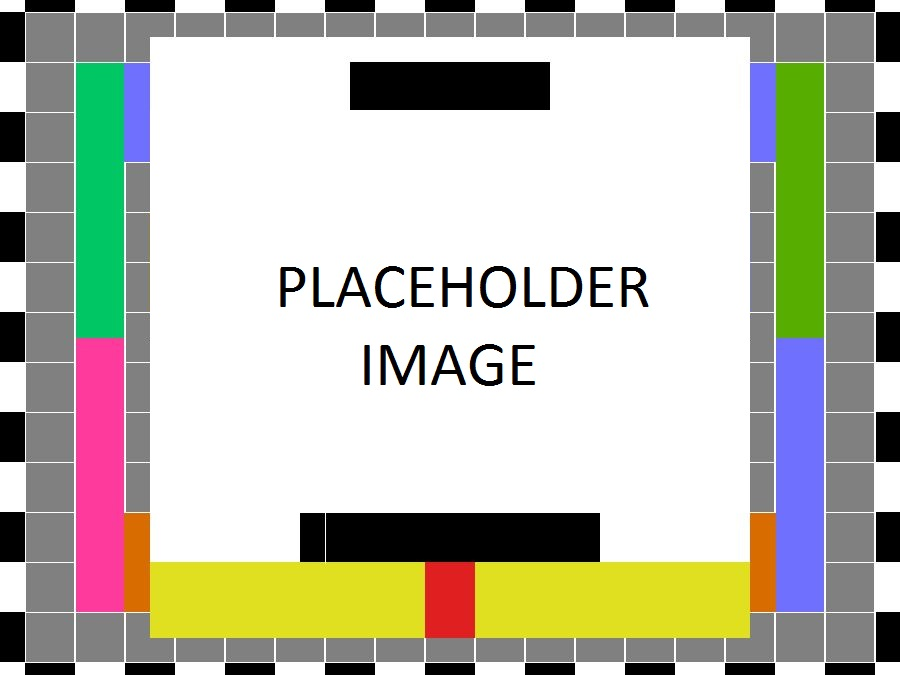
\includegraphics[width=0.60\textwidth]{images/test_image}
    \caption{X conceptual drawing}
\end{figure}

\newpage
\section{Product Description}
A vest using fine-tuned vibrations to allow those who cannot hear sound to feel it through their body instead. This integrated signal processing to separate the low, mid, and high frequencies sound creates. These frequencies are then sent to bass shakers throughout the vest to accurately deliver sound to the body via vibrations. Also, with my background in music, the feelings that the vest delivers will be extremely accurate to any user.

\subsection{Features \& Functions}
A unique design, a padded vest will be presented. This vest will have bass shakers integrated into the vest. It will have an intensity knob allowing the user to increase or decrease the vibrations that they feel. Will have an audio jack to plug in media player. With have integrated power pack. Will have integrated computer which will be the brain of the functionality. Bluetooth connection integration may also be an option.

\subsection{Product Interfaces}
Will have a knob integrated into the vest to Increase/decrease vibration intensityons, panels, etc. Refer to the critical external inputs and outputs described in the paragraph above.

\newpage
\section{Customer Requirements}
The vest has some features that have been demanded by the customer. These features will be made use of by the user and determines their satisfaction of the prodct  The details of the features are described below. These features are subject to change for the moment and will be updated but not without general consensus from the team.
\subsection{The vest shall not be bulky}
\subsubsection{Description}
The vest should not be heavy for the user when it is worn.A detailed description of the feature/function that satisfies the requirement. This is so that the user would be able to carry it arround without feeling  inconvenienced.
\subsubsection{Source}
Customer 
\subsubsection{Priority}
High

\subsection{The vest should be stylish}
\subsubsection{Description}
The vest should look good to the eye
Detailed requirement description...
\subsubsection{Source}
Customer
\subsubsection{Priority}
Medium

\subsection{The intensity of vibration should be changeable }
\subsubsection{Description}
The user should be able to increase and decrease the general vibration of the vest
Detailed requirement description...
\subsubsection{Source}
Customer
\subsubsection{Priority}
Medium

\subsection{The vest should be safe}
\subsubsection{Description}
The user should be able to use the vest without any hazards
Detailed requirement description...
\subsubsection{Source} 
Customer
\subsubsection{Priority}
Critical

\newpage
\section{Packaging Requirements}
Include a header paragraph here. Packaging requirements are those requirements that identify how the delivered product will be packaged for delivery to the end-user; or how it will "look" when finished and delivered. For example, you might specify that the software required for operation will be pre-loaded on the hard drive, delivered on CD/DVD, or available via download. Software might be customer installable, or not, etc. Hardware components could be all in a single package, provided as a "bag of parts" to be assembled/installed by the user, painted a certain color, logos affixed, etc. Care should be taken not to duplicate requirements found in other sections of this document.

\subsection{Requirement Name}
\subsubsection{Description}
Detailed requirement description...
\subsubsection{Source}
Source
\subsubsection{Constraints}
Detailed description of applicable constraints...
\subsubsection{Standards}
List of applicable standards
\subsubsection{Priority}
Priority
\newpage
\section{Performance Requirements}
Include a header paragraph specific to your product here. Performance requirements address items such as: how fast specific critical operations must complete; how long it takes to start/stop activities; how long the battery must last; maximum time it must take to set up; etc.

\subsection{Requirement Name}
\subsubsection{Description}
Detailed requirement description...
\subsubsection{Source}
Source
\subsubsection{Constraints}
Detailed description of applicable constraints...
\subsubsection{Standards}
List of applicable standards
\subsubsection{Priority}
Priority
\newpage
\section{Safety Requirements}
Include a header paragraph specific to your product here. Safety requirements might address items specific to your product such as: no exposure to toxic chemicals; lack of sharp edges that could harm a user; no breakable glass in the enclosure; no direct eye exposure to infrared/laser beams; packaging/grounding of electrical connections to avoid shock; etc.

\subsection{Laboratory equipment lockout/tagout (LOTO) procedures}
\subsubsection{Description}
Any fabrication equipment provided used in the development of the project shall be used in accordance with OSHA standard LOTO procedures. Locks and tags are installed on all equipment items that present use hazards, and ONLY the course instructor or designated teaching assistants may remove a lock. All locks will be immediately replaced once the equipment is no longer in use.
\subsubsection{Source}
CSE Senior Design laboratory policy
\subsubsection{Constraints}
Equipment usage, due to lock removal policies, will be limited to availability of the course instructor and designed teaching assistants.
\subsubsection{Standards}
Occupational Safety and Health Standards 1910.147 - The control of hazardous energy (lockout/tagout).
\subsubsection{Priority}
Critical

\subsection{National Electric Code (NEC) wiring compliance}
\subsubsection{Description}
Any electrical wiring must be completed in compliance with all requirements specified in the National Electric Code. This includes wire runs, insulation, grounding, enclosures, over-current protection, and all other specifications.
\subsubsection{Source}
CSE Senior Design laboratory policy
\subsubsection{Constraints}
High voltage power sources, as defined in NFPA 70, will be avoided as much as possible in order to minimize potential hazards.
\subsubsection{Standards}
NFPA 70
\subsubsection{Priority}
Critical

\subsection{RIA robotic manipulator safety standards}
\subsubsection{Description}
Robotic manipulators, if used, will either housed in a compliant lockout cell with all required safety interlocks, or certified as a "collaborative" unit from the manufacturer.
\subsubsection{Source}
CSE Senior Design laboratory policy
\subsubsection{Constraints}
Collaborative robotic manipulators will be preferred over non-collaborative units in order to minimize potential hazards. Sourcing and use of any required safety interlock mechanisms will be the responsibility of the engineering team.
\subsubsection{Standards}
ANSI/RIA R15.06-2012 American National Standard for Industrial Robots and Robot Systems, RIA TR15.606-2016 Collaborative Robots
\subsubsection{Priority}
Critical

\newpage
\section{Maintenance \& Support Requirements}
Include a header paragraph specific to your product here. Maintenance and support requirements address items specific to the ongoing maintenance and support of your product after delivery. Think of these requirements as if you were the ones who would be responsible for caring for customers/end user after the product is delivered in its final form and in use "in the field". What would you require to do this job? Specify items such as: where, how and who must be able to maintain the product to correct errors, hardware failures, etc.; required support/troubleshooting manuals/guides; availability/documentation of source code; related technical documentation that must be available for maintainers; specific/unique tools required for maintenance; specific software/environment required for maintenance; etc.

\subsection{Requirement Name}
\subsubsection{Description}
Detailed requirement description...
\subsubsection{Source}
Source
\subsubsection{Constraints}
Detailed description of applicable constraints...
\subsubsection{Standards}
List of applicable standards
\subsubsection{Priority}
Priority
\newpage
\section{Other Requirements}
Include a header paragraph specific to your product here. In this section specify anything else that is required for the product to be deemed complete. Include requirements related to customer setup and configuration if not specified in a previous requirement. Add any known requirements related to product architecture/design, such as modularity, extensibility (for future enhancements), or adaptation for a specific programming language. Consider requirements such as portability of your source code to various platforms (Windows, Linux, Unix Mac OS, etc.).

\subsection{Requirement Name}
\subsubsection{Description}
Detailed requirement description...
\subsubsection{Source}
Source
\subsubsection{Constraints}
Detailed description of applicable constraints...
\subsubsection{Standards}
List of applicable standards
\subsubsection{Priority}
Priority
\newpage
\section{Future Items}
In this last section, you will reiterate all requirements that are listed as priority 5. This is repetitive, but necessary as a concise statement of features/functions that were considered/discussed and documented herein, but will NOT be addressed in the prototype version of the product due to constraints of budget, time, skills, technology, feasibility analysis, etc. Use the following format for this section.

\subsection{Requirement Name}
\subsubsection{Description}
Detailed requirement description...
\subsubsection{Source}
Source
\subsubsection{Constraints}
Detailed description of applicable constraints...
\subsubsection{Standards}
List of applicable standards
\subsubsection{Priority}
Priority
\newpage

%%% References
\bibliographystyle{plain}
\bibliographystyle{reference/IEEEtran_custom}
\bibliography{reference/refs}{}

\end{document}